\documentclass[12pt]{article}
\usepackage[utf8]{inputenc}
\usepackage[brazil]{babel}
\usepackage{geometry}
\usepackage{graphicx}
\usepackage{titlesec}
\usepackage{enumitem}
\usepackage{hyperref}
\usepackage{longtable}
\usepackage{xcolor}
\usepackage{anyfontsize}


\geometry{a4paper, margin=2.5cm}

\titleformat{\section}{\normalfont\Large\bfseries}{\thesection}{1em}{}
\titleformat{\subsection}{\normalfont\large\bfseries}{\thesubsection}{1em}{}

\begin{document}

\begin{flushleft}
    {\fontsize{30}{22}\selectfont \textcolor{blue}{Corigge}}\\[2cm]
    {\fontsize{22}{22}\selectfont \textbf{VISÃO DO PRODUTO E PROJETO}}\\[2cm]
    {\fontsize{16}{22}\selectfont Versão 0.2}\\[2cm]
\end{flushleft}

\vfill
\section*{Histórico de Revisão}
\begin{longtable}{|l|l|p{8cm}|l|}
\hline
\textbf{Data} & \textbf{Versão} & \textbf{Descrição} & \textbf{Autor} \\
\hline
05/04/2025& 0.1 & Completando seções 1 e 2  & Otávio\\
\hline
08/04/2025& 0.2 & Corrigindo erros apontados na versão 0.1 & Otávio\\
\hline
& & & \\
\hline
& & & \\
\hline
\end{longtable}

\thispagestyle{empty}
\newpage
\newpage


\section{Cenário Atual do Cliente e do Negócio}

\subsection{Introdução ao Negócio e Contexto}
A Guia do PAS é uma empresa especializada na preparação de estudantes para o Programa de Avaliação Seriada (PAS) da Universidade de Brasília (UnB), um dos processos seletivos mais concorridos do país. Atuando no setor educacional, a empresa oferece conteúdos direcionados, simulados, correções comentadas, aulas ao vivo e materiais exclusivos, com foco na aprovação dos alunos. A empresa, nos últimos anos, também tem expandido seu mercado para o abranger o atendimento à outras instituições de ensino, oferecendo a aplicação de simulados, listas de exercícios personalizadas e controle de desempenho dos alunos. Além disso, a empresa tem buscado expandir sua atuação para outros processos seletivos além do PAS, visando aumentar sua base de clientes e diversificar seus serviços.

A empresa já tentou desenvolver uma solução anteriormente, também chamada Corigge, mas esta primeira versão apresentou diversos problemas técnicos que comprometeram sua utilização efetiva. O sistema anterior, que era uma aplicação web, necessitava de manutenção constante e apresentava várias limitações operacionais: o servidor precisava estar sempre ativo em um computador específico com boa capacidade de processamento, onde um script Python precisava ser executado manualmente para permitir que outros usuários acessassem o sistema. Além disso, o sistema apresentava instabilidades frequentes, com múltiplas ocorrências de crashes tanto no servidor quanto na aplicação, sem mecanismos de auto-recuperação. A necessidade de ajustes manuais de parâmetros pelos usuários finais também se mostrou um obstáculo significativo para a adoção do sistema. A funcionalidade do sistema anterior era limitada apenas à identificação das respostas dos alunos, sem oferecer recursos adicionais como análise de desempenho, geração de relatórios ou personalização de gabaritos.


\subsection{Identificação da Oportunidade ou Problema}
Com o crescimento da base de usuários e o aumento no número de clientes B2B buscando a realização de simulados em suas escolas, percebeu-se algumas dificuldades na obtenção das respostas dos alunos, na inserção desses dados no banco de dados da empresa e a visualização desses dados de forma efetiva pelos coordenadores das escolas parceiras. Após a aplicação do simulado é necessário registrar as respostas de cada aluno e associar esses dados com a matrícula do aluno, utilizando desses dados em uma planilha .csv para ser cadastrada no sistema da empresa. Mesmo fazendo uso de serviços de outras empresas para realizar essa identificação dos gabaritos, essas soluções eram demoradas e muito custosas (demorando mais de um mês para receber os resultados e custando em média R\$1500.00 por simulado), não tendo sido possível encontrar uma solução rápida, de fácil uso e barata para a realização de grandes simulados ou de simulados em várias escolas em um curto período de tempo. 

Diante dessas experiências anteriores e da necessidade de uma solução mais robusta, a empresa busca o desenvolvimento de uma nova versão do sistema como uma aplicação desktop, que permita a correção automática dos gabaritos de forma eficiente e rápida, desejando também oferecer esse serviço para outras instituições de ensino não associadas à empresa.

\begin{figure}[ht!]
    \centering
    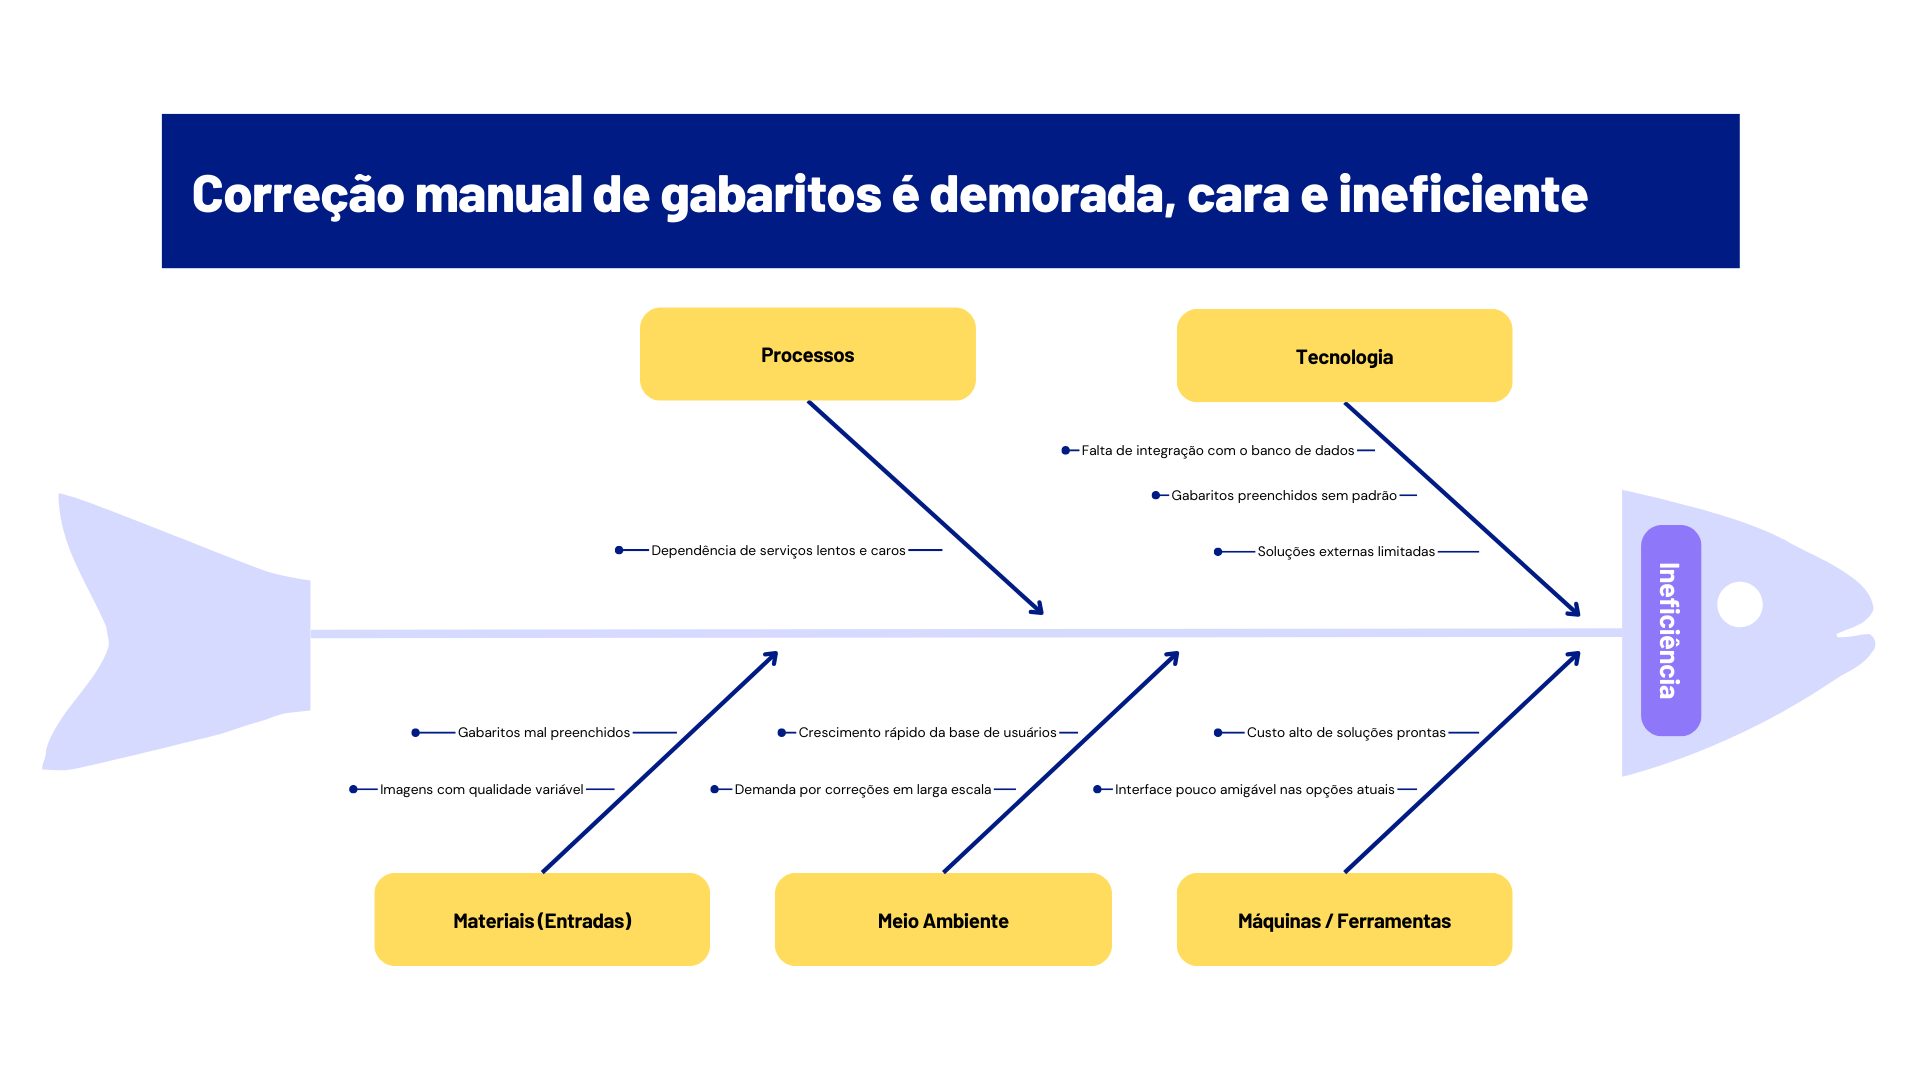
\includegraphics[width=0.9\textwidth]{diagrama_fishbone.png}
    \caption{Diagrama de Ishikawa (Fishbone) com os principais desafios do projeto}
    \label{fig:fishbone}
\end{figure}


\subsection{Desafios do Projeto}

Os principais desafios do projeto são: A utilização e parametrização de ferramentas de CV (Visão computacional) para a identificação das respostas dos alunos, a não padronização dos gabaritos preenchidos pelos alunos, a não familiaridade de alguns membros da equipe com as ferramentas a serem utilizadas, a criação de um design amigável, eficiente e intuitivo para a utilização pelos membros da empresa, e o empacotamento das ferramentas necessárias para integrar o CV em uma aplicação multiplataforma em flutter.

\subsection{Segmentação de Clientes}
O público alvo atual da empresa são alunos do ensino médio e alunos de cursinhos que buscam uma preparação estratégica e eficiente para o PAS, além de instituições de ensino que desejam ter uma preparação mais específica para o PAS e simulados personalizados para esta preparação.

O perfil dos alunos é de jovens entre 15 e 20 anos, que buscam uma preparação diferenciada para o PAS, com foco em resultados e aprovação. Eles valorizam a qualidade do conteúdo, a eficiência dos simulados e a possibilidade de acompanhar seu desempenho ao longo do tempo.

O perfil dos coordenadores das instituições de ensino são profissionais com formação superior, que atuam na área de educação e buscam soluções tecnológicas para otimizar a gestão acadêmica e melhorar a experiência dos alunos. Eles valorizam a eficiência e a facilidade de uso das ferramentas que utilizam.

\section{Solução Proposta}

\subsection{Objetivos do Produto}

O objetivo principal do produto é aumentar a eficiência operacional da empresa, agilizando o processo de digitalização dos gabaritos, identificação das respostas e produção de análises individuais e de grupos de alunos, além de aumentar os lucros da empresa com a venda do serviço para outras instituições de ensino e removendo as dificuldades encontradas com o software anterior.


\subsection{Características da Solução}
O produto será um aplicativo desktop multiplataforma (Windows, Linux e MacOS) que deve ser capaz de processar imagens de gabaritos preenchidos pelos alunos, identificar as respostas dadas pelos alunos em cada questão, identificar a matrícula do aluno, comparar as respostas com o gabarito correto, gerar relatórios detalhados (com o desempenho do aluno — incluindo notas, acertos e erros —, comparações entre alunos, comparações entre grupos de alunos e dados estatísticos de cada questão). O produto também deve ser capaz de gerar templates de gabaritos e permitir a personalização dos gabaritos de acordo com as necessidades de cada instituição de ensino. Além disso, o produto também deve permitir a exportação dos dados e relatórios para arquivos .csv e .pdf, para facilitar a integração com outros sistemas e a análise dos dados. A escolha por uma aplicação desktop também visa facilitar o processo de desenvolvimento, permitindo que a equipe de desenvolvimento da empresa adicione mais funcionalidades ao longo do tempo de forma ágil e eficiente.


\subsection{Tecnologias a Serem Utilizadas}

As tecnologias a serem utilizadas para o desenvolvimento do produto são:

\begin{itemize}
    \item Frontend: Dart + Flutter
    \item Identificação de imagem local: Python + OpenCV
    \item Backend: Typescript + Express.js
    \item Banco de dados: Supabase (PostgreSQL)
    \item Hospedagem: Azure + VM Linux
\end{itemize}

\subsection{Pesquisa de Mercado e Análise Competitiva}

\begin{itemize}
    \item \textbf{RemarkOffice}: Possui um preço muito alto (\$1,195.00), não oferece a possibilidade de personalização dos gabaritos e não possui precificação por gabarito analisado (deixando o serviço mais barato para pequenas empresas). 
    \item \textbf{Gradepen}: É gratuito mas pouco conhecido. Também não oferece estatísticas de desempenho do aluno, apenas a correção do gabarito. Também não oferece a possibilidade de personalização dos gabaritos.
    \item \textbf{Prova Fácil}: Custa \$0.15 por correção, não oferece estatísticas de desempenho do aluno, apenas a correção do gabarito. Também não oferece a possibilidade de personalização dos gabaritos.
\end{itemize}



\subsection{Análise de Viabilidade}

A viabilidade técnica do projeto é alta, uma vez que a equipe possui experiência em desenvolvimento de plataformas similares e familiaridade com as tecnologias propostas como \textbf{Flutter}, \textbf{PostgreSQL}, \textbf{Typescript} e a com os \textbf{serviços de cloud} a serem utilizados. O prazo é de 3 meses para o desevolvimento da solução, o que é viável considerando a complexidade do projeto e a experiência da equipe. O custo estimado para o desenvolvimento é de R\$1,000.00 para eventuais pagamentos de serviços como o banco de dados e hosteamento dos servidores backend durante o desenvolvimento, o que é viável considerando a demanda do mercado e o preço cobrado pelos concorrentes. O retorno financeiro inicial esperado é de R\$1,000.00 por mês (uma estimativa baixa considerando apenas 2000 correções por mês à R\$0.50 por correção, o que é facilmente atingível dado o crescimento atual da empresa no mercado de Brasília e a possibilidade de oferecimento desse serviço para diversas empresas de educação do país), considerando a venda do serviço para outras instituições de ensino e o crescimento da confiabilidade na empresa, o que permite o oferecimento do serviço para várias instituições de Brasília.

\subsection{Impacto da Solução}

A solução proposta terá um impacto significativo na eficiência operacional da empresa, reduzindo o tempo (de um mês para algumas horas) e os custos associados (de R\$5,00 para menos de R\$1,00 por correção) à correção de gabaritos. Além disso, a solução permitirá a venda desse serviço para outras instituições de ensino, aumentando a receita da empresa em pelo menos R\$12.000,00 por ano e expandindo sua atuação no mercado educacional, expandindo a influência da empresa no mercado de preparação para o PAS. A solução também melhorará a experiência do usuário, proporcionando resultados mais rápidos (análise de 100 gabaritos por minuto) e precisos, além de relatórios detalhados sobre o desempenho dos alunos. 

\section{Estratégias de Engenharia de Software}

\subsection{Estratégia Priorizada}


\subsection{Quadro Comparativo}


\subsection{Justificativa}

\section{Cronograma e Entregas}



\section{Interação entre Equipe e Cliente}

\subsection{Composição da Equipe}


\subsection{Comunicação}


\subsection{Processo de Validação}


\section{Lições Aprendidas}

\subsection{Unidade 1}

\subsection{Unidade 2}

\subsection{Unidade 3}

\subsection{Unidade 4}



\section{Referências Bibliográficas}

\end{document}
